\documentclass{article}
\usepackage[italian]{babel}
\usepackage[T1]{fontenc}
\usepackage{graphicx}
\usepackage[utf8x]{inputenc}
\usepackage{amsmath}
\usepackage{amsthm}
\usepackage{hyperref}
\date{}
\author{Francesco Sacco Lorenzo Cavuoti}
\title{Caratteristiche porte logiche e semplici circuiti logici}

\begin{document}
	\maketitle
	\paragraph{0)}
	Lo scopo dell'esperienza è misurare le caratteristiche statiche e dinamiche delle porte NOT contenute nell’integrato SN74LS04 (HEX Inverter) e costruire semplici circuiti logici con le porte NAND.
	
	\paragraph{1a)}
	Si è montato il circuito in figura \ref{fig:circuito-1} e si è alimentato con $V_{CC}=4.7\pm0.2$ V usando solo un generatore. Successivamente si è fatta variare la resistenza del potenziometro e si è segnato $V_{in}$ e $V_{out}$ per ciascuna posizione del potenziometro, i dati sono riportati in tabella e nel grafico in figura
	
	
\begin{figure}
	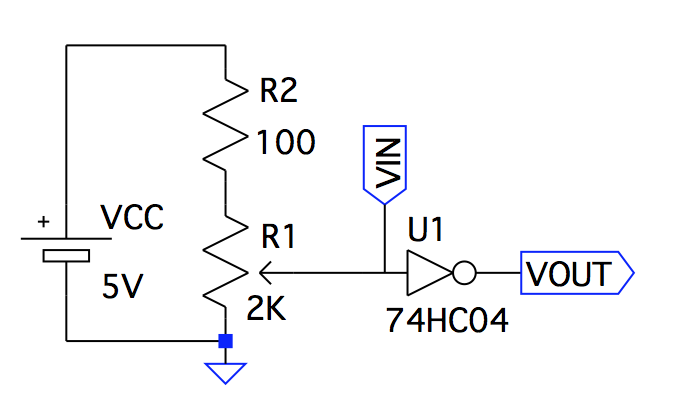
\includegraphics[width=0.8\linewidth]{figure/circuito1}
	\caption{Circuito usato per misurare VIH, VIL, VOH, VOL}
	\label{fig:circuito-1}
\end{figure}

\begin{table}
	\begin{tabular}{cc}
		\hline
		$V_{in}$ & $V_{out}$ \\
		\hline
		$(1.0\pm0.01)\times 10^{-2}$ & $4.31\pm0.02$ \\
		$0.49\pm0.003$ & $4.31\pm0.02$ \\
		$0.99\pm0.005$ & $4.24\pm0.02$ \\
		$1.33\pm0.007$ & $2.83\pm0.02$ \\
		$1.51\pm0.008$ & $0.97\pm0.005$ \\
		$2.03\pm0.01$ & $0.11\pm0.0006$ \\
		$2.49\pm0.02$ & $0.11\pm0.0006$ \\
		$3.06\pm0.02$ & $0.11\pm0.0006$ \\
		$3.46\pm0.02$ & $0.11\pm0.0006$ \\
		$3.99\pm0.02$ & $0.11\pm0.0006$ \\
		$4.43\pm0.02$ & $0.11\pm0.0006$ \\
		$4.67\pm0.03$ & $0.11\pm0.0006$ \\
		\hline
	\end{tabular}
\end{table}




\end{document}